\chapter{Część kliencka aplikacji}

Część kliencka naszej aplikacji została oparta o javascriptowy framwork Ext JS. Jest to rozbudowany pakiet do tworzenia nowoczesnych aplikacji internetowych. Udostępnia funkcje do zarządzania elementami drzewa DOM, oraz szereg własnych komponentów graficznych tj. panele, tabelki, formularze etc. Biblioteka posiada również szerokie wsparcie dla technologii AJAX. Ext JS został stworzony z myślą o tworzeniu rozbudowanych aplikacji i dlatego twórcy pomyśleli o architekturze, która pozwoli w naturalny i logiczny sposób zorganizować kod programu. Struktura aplikacji opiera się o schemat MVC. Twórcy Ext JS zalecają pewien schemat hierarchii katalogów uwzględniający podział projektu na warstwy. Przykład organizacji aplikacji:

\begin{figure}
	\centering
	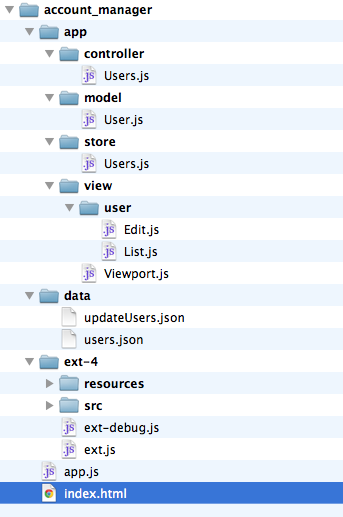
\includegraphics[scale=0.7]{images/struktura_folderow.png}
	\caption{Struktura folderów aplikacji}
\end{figure}

\section{Warstwa modelu}

Definiuje klasy będące odwzorowaniem klas języka Java, które otrzymujemy w odpowiedzi od serwera. W klasach modelu wykonujemy konwersję surowych danych do czytelnego formatu jeżeli jest taka potrzeba. Na tym poziomie możemy również wprowadzić walidację pól. Ext JS wspiera architekturę REST dzięki temu w klasach modelu podając adres URL do zasobów otrzymamy gotowe funkcje zapisu, odczytu, modyfikacji i usuwania danych. Przeanalizujmy przykład z naszego projektu:

Ext.define('RevCommunity.model.Category', {
    extend: 'Ext.data.Model',
    fields: [
		'name',
		'nodeId',
		'filters'
	 ],
     idProperty:'nodeId',
     proxy: {
        type: 'rest',
        url : 'rest/categories'
    }
});


Powyższy kod implementuje klasę modelu Category. Dzięki definicji obiektu proxy zarządzanie naszymi danymi staje się banalnie proste. Przykładowo w celu zapisania nowej kategorii wystarczy:

var category = Ext.create('Category', {name: 'Komputery'});

category.save(); // wywołanie zapytania metodą POST pod adres 'rest/categories'
// treść zapytania to definicja obiektu kategorii w formacie JSON

Jeżeli wykonamy metodę save na obiekcie, który posiada już przypisany identyfikator(w naszym przypadku pole nodeId), to metodą zapytania będzie PUT.
Do dyspozycji mamy również metody destroy(usuwanie elementu), oraz load(pobieranie elemntu).

Kolejnym elementem zaliczającym się do tej warstwy są klasy Store służące do zarządzania grupami obiektów. Wykorzystuje się je przy ładowaniu danych do komponentów np. tabel. 
Klasy Store pozwalają również filtrować i sortować dane.

\section{Warstwa widoku}

Na widok aplikacji składają się komponenty graficzne tj. panele, tabele, drzewa i formularze. Biblioteka pozwala nam rozszerzać komponenty graficzne tworząc własne, dzięki temu możemy je dostosować do własnych potrzeb i wykorzystywać w wielu miejscach(również w innych aplikacjach). Bardzo przydatnym elementem Ext JS jest mechanizm szablonów(Ext.XTemplate). Pozwala on tworzyć wygląd komponentów z wykorzystaniem języka HTML i specjalnych znaczników framework'a Ext JS. Zazwyczaj szablony służą do definicji wyglądu list elementów. Komponent, w którym używamy szablonu wiążemy z konkretnym modelem. Gdy spróbujemy załadować dane do komponentu model wywoła odpowiednie zapytanie do serwera w celu pobrania danych. Następnie zwrócona kolekcja zostanie przetworzona przez szablon. W szablonie możemy odwoływać się do pól modelu, iterować po kolekcjach elementów, oraz wykorzystywać warunki logiczne. Spójrzmy na prosty przykład szablonu listy subskrybowanych użytkowników:
 

<p class="rev-header">Subskrupcje</p>
<tpl for=".">
    <div class="rev-user-subscription-item">
      <img src="{user.image}" width="18"/><span>{user.fullName} ({newNotifications})</span>
    </div>
</tpl>

Widok naszego komponentu w całości definiuje powyższy szablon. Zaczynamy od wstawienia nagłówka "Subskrypcje" jako zwykły paragraf HTML. Niżej widzimy znacznik 'tpl', który udostępnia rozszerzenia szablonów. W tym przypadku będziemy iterować po kolekcji elementów załadowanej do komponentu. Następnie mamy definicje elementów HTML zawierających znaczniki odwołujące się do pól modelu. Jednym z pól modelu jest obiekt user. Możemy odwoływać się do jego właściwości poprzez znak '.'. W połączeniu z definicją stylów CSS otrzymujemy następujący efekt:

 


\section{Warstwa kontrolerów}

Aby nasza aplikacja zaczęła "żyć" musimy zdefiniować zachodzące w nie zdarzenia i ich obsługę. Do tego służą kontrolery. Są to klasy w których umieszczamy instrukcję w typu: gdy na komponencie ... wydarzy się ... wykonaj ... . Przykładowo w kontrolerach umieszczamy obsługę kliknięć przycisków, zdarzeń załadowania danych, lub edycji pól formularzy. Ciekawy jest sposób wiązania komponentu z funkcją obsługi zdarzenia. Pierwszą istotną rzeczą, którą musimy wykonać to zidentyfikowanie komponentu dla którego będziemy definiować zdarzenie. Do tego celu wykorzystujemy mechanizm Ext Js - ComponentQuery. Jest to język zapytań pozwalający na wyszukiwanie komponentów na podstawie aliasów, identyfikatorów, powiązań z innymi komponentami, oraz wartości ich atrybutów. Każda klasa powinna posiadać unikalny w ramach aplikacji alias. Alias ten upraszcza tworzenie obiektów danej klasy(nie musimy podawać pełnej nazwy klasy), oraz znacznie ułatwia tworzenie zapytań. Spójrzmy na przykład: 

revhtmleditor  > toolbar button[action=addVideoWin]

Zapytanie zostanie przetworzone w następujący sposób:
•	wyszukanie wszystkich komponentów na stronie posiadających alias 'revhtmleditor'
•	wśród bezpośrednich dzieci znalezionych wcześniej komponentów wybierzemy tylko elementy typu toolbar ( gdyby nie znak '>' wyszukiwanie zagłębiałoby się rekurencyjnie)
•	w znalezionych toolbar'ach szukamy tylko przycisków, mających atrybut action ustawiony na wartość addVideoWin

Tak elastyczny mechanizm wyszukiwania pozwala znaleźć każdy komponent.
Kolejnym krokiem jest wybranie zdarzenia dla znalezionego komponentu. Ext Js określił dla każdego komponentu wyczerpującą listę dostępnych zdarzeń. Naszym zadaniem jest ich przypisanie do funkcji javascriptowych i implementacji obsługi.

Naszym rozszerzeniem powyższej architektury jest dodanie warstwy usług, której zadanie jest analogiczne do jej serwerowego odpowiednika. Stworzenie klas usług po stronie klienta miało na celu wyciągniecie implementacji z klas kontrolerów po to, aby lepiej zorganizować kod i umożliwić korzystanie z przydatnych funkcji w wielu miejscach. Pamiętajmy, że kontrolery są mocno związane z komponentami, natomiast klasy usług są podzielone według obszaru, którego dotyczą np. produktów, recenzji. Dlatego kontrolery zajmują się przetworzeniem danych do odpowiedniego formatu wymaganego przez klasy usług, nie implementują bezpośrednio żadnych operacji.


